\documentclass[12pt,english]{article}
\usepackage[T1]{fontenc}
\usepackage[latin1]{inputenc}
\usepackage{times}
\usepackage{a4wide}
\usepackage{graphicx}
\usepackage{babel}
\usepackage[pdftex,bookmarks=false,linkbordercolor={0.5 1 0.5}]{hyperref}

\newcommand{\st}{{\tt sta\-tist} }

\begin{document}

\title{STATIST 1.4.1\\User Manual}
\author{Jakson Alves de Aquino\\
{\small {\tt jalvesaq@gmail.com}}}
\date{September 5, 2006}

\maketitle

\tableofcontents
 
\section{Introduction}

{\tt Statist} is an easy to use, light weight statistics
program.  Everything is in an interactive menu: you have
just to choose what you need. {\tt Statist} is Free Software
under GNU GPL and comes with absolutely no guarantee. 

This manual is an incomplete and non literal translation
from the original text written by Dirk Melcher, but with the
addition of new material. I'm grateful to Bernhard Reiter
for his suggestions of improvements to this document.

\section{Warnings for Windows users}

Users on GNU/Linux are much more accustomed to use console
applications.  One helpful feature is the command line
completion, where a long file name will be completed after
typing the first letters and then pressing tab.  The
terminal emulators, where you type in commands, can save and
scroll over many lines that have come by.  And, the most
important, GNU/Linux is Free Software where anybody can
inspect what the computer does and many people can fix bugs
to make this more secure.  Please, as soon as you can, try
\st on a Free Software operating system like GNU/Linux or
FreeBSD.

To create graphics with \st you will need a version of {\tt
gnuplot} that comes with {\tt pgnuplot}. Under Windows, you
can't send commands to {\tt gnuplot} through {\tt sta\-tist}, as it is
possible under Linux, but you can type the commands in the
{\tt gnuplot} window.

Be careful: Don't close the {\tt gnuplot} window.  You can
close only the graphic! If you close the {\tt gnuplot}
window you will have to restart \st to be able to create
graphics again.

Some software used to manipulated data files aren't part of
{\tt sta\-tist}, but they are available for Windows. Please, search the
Internet, looking for the package gnucoreutils, which is one
of the GnuWin32 packages. Note, however that their
installation and use might not be trivial for a Windows
user.  Like {\tt sta\-tist}, they are easier to use in a
Linux terminal emulator than in a DOS window.

The \st documentation can be found at {\tt
C:$\backslash$Program Files$\backslash$statist}, where there
is also a sample configuration file for {\tt sta\-tist}. You
can rename it to {\tt statistrc.txt} and edit it according
to your preferences.

Unfortunately, \st can't produce colorized output under DOS.

\section{Installation from source code}

\begin{enumerate}

\item Open a terminal.

\item Unpack the source code, compile the program, and
become root to install it. That is, type:

\end{enumerate}

\begin{verbatim}
    tar -xvzf statist-1.4.1.tar.gz
    cd statist-1.4.1
    make
    # optional, if you have "check" installed
    make check

    # install for all users as root
    su -
    cd path-to/statist-1.4.1
    make install
    exit

\end{verbatim}

This is the default installation that should work in most
GNU/Linux distributions. If the above instructions are not
enough for your case, please see the file README for details
on how to install \st from source code.

\section{Invocation}

You can simply type:
\begin{verbatim}
    statist data_file
\end{verbatim}

However there are also some options that you might find
useful, and, then, the invocation will be:

\begin{verbatim}
 statist [ options ] data_file [ options ] 
\end{verbatim}

The only option that you need to memorise is {\tt {-}-help},
or simply {\tt -h}, which will output the list of options.

You can also create and edit the file {\verb ~/.statistrc }
and set some options there.  If you have root privileges,
you can also create the file {\tt /etc/statistrc}.  Options
passed by the command line override the ones read from the
{\tt statistrc} file.  You can find a sample {\tt statistrc}
in the documentation directory (usually {\tt
/usr/share/doc/statist}). Finally, if you choose the menu
item {\em Preferences}, you can modify some options during \st
execution.

\section{Menu}

The program has a simple menu that makes it very easy to
use. There is no need of remembering commands. Typing `0'
you go to the next higher menu-level, or finishes the
program if you already are in the {\em Main menu}. One tip
is important: if you have chosen a menu entry by mistake,
you can always cancel the process by pressing the <Return>
key before entering any value or answering any question.
Then, the last menu will be printed again. 

If you choose a statistical procedure from the menu, you
will be asked to choose the variables. Often, it's not
necessary to type the entire name of a column when inputting
variable names for analyzes. For example, if you have a
column named 

\begin{center}
this\_really\_is\_a\_big\_name
\end{center}

\noindent and there is no other column starting with the
letter `t', you can simply type `t'. Finally, if you want to
select all columns, you might simply type ``all'' as the
name of the first column.

Actually, the whole process is self-explanatory, and you
would be able to use the program even without reading this
short explanation.
%Click <a href="menulist.html">here</a> to see the complete
%menu.

 
\section{Statist and Gnuplot}

Gnuplot is an interactive program that makes graphical
presentations from data and functions, and \st creates {\tt
gnuplot} graphics for some functions. Normally, you will not
have to open {\tt gnuplot} manually. The prerequisite to use
it is simply that the program is installed and in the PATH.

If you know {\tt gnuplot} syntax, you can refine or
personalize your graphics, inputting {\tt gnu\-plot}
commands. To do that, choose the menu option {\em
Miscellaneous} {\textbar} {\em Enter gnuplot commands}. You can change many
things in the graphic, like line colors and types, axes
labels etc... Even if you don't know {\tt gnuplot} syntax,
you can at least change the graphics title and axes labels
because a list of the last commands sent to {\tt gnuplot}
will be printed in the screen.  The changes will be applied
to the current graphic being displayed with the {\tt
gnuplot} command ``replot''. 

The {\tt gnuplot} graphics can be disabled invoking the
program with the option {\verb --noplot }. This can be
useful if you, for example, will work with batch processing
or if your database is too big and, thus, {\tt gnuplot}
graphics are being generated too slowly.

\subsection{Box-plot}

You probably will have no problem interpreting \st graphics.
The only one that might need some explanation is the {\em
Box-and-Whisker Plot}. The picture below shows the meaning
of each piece of this graphic:

\begin{center}
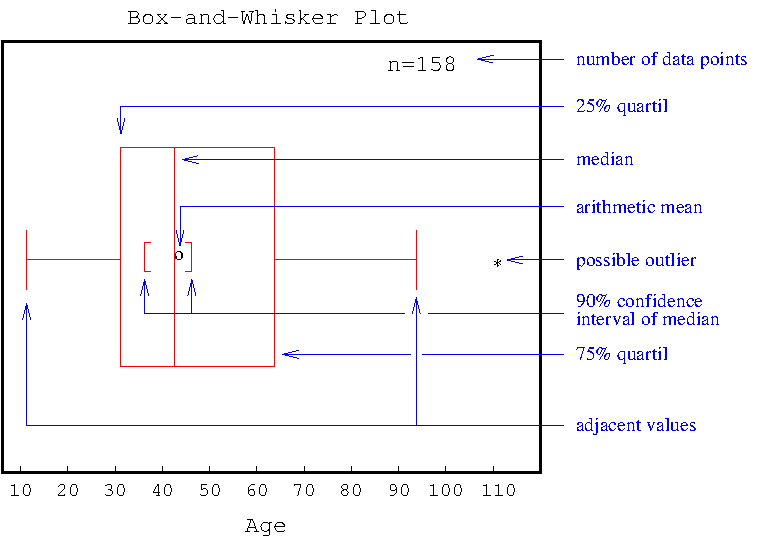
\includegraphics{boxplot-en}
\end{center}

\subsection{UTF-8}

You might experience some problems with \st graphics
made through gnuplot if your locale environment is set to
UTF-8 and your language has non-ascii characters. The
problem is that gnuplot will normally interpret titles and
labels as they were encoded in a single-byte character set,
like ISO-8859-1 (Latin 1), even if the terminal emulator
charmap is set to UTF-8. It's possible to mix letters of
different character sets (Greek and Latin 1, for example) in
a single graphic. Please, access the web page below to know
the details:

\href{http://statist.wald.intevation.org/utf8.html}
{http://statist.wald.intevation.org/utf8.html}

\section{Data}

\subsection{The file format}

{\tt Statist} reads data from simple ASCII files (text
files).  If the program is not invoked with an ASCII file
name, it will immediately asks for the name of a data-file.
Without data-file, there is nothing to do, unless you
declare the option \verb --nofile  while invoking the
program in order to use the keyboard to input data manually
(choose from the menu: {\em Data management} {\textbar} {\em Read column
from terminal}). However, only rarely it is reasonable to do
this. It would be more comfortable to use a text editor or a
spreadsheet program like {\em OpenOffice Calc} and {\em
Gnumeric}. In this case, save the file as .csv.

But be careful, because \st always uses a dot as decimal
delimiter while working with data files. If the decimal
delimiter in your language is a comma, \st might fail to
correctly read the file. Thus, before typing your
data, you can try to open the spreadsheet program in a
terminal with locale set to ``C'', as below:

\begin{verbatim}
  export LC_ALL=C
  oocalc &
\end{verbatim}

If you really need to use a data file with commas as decimal
delimiters, \st will convert each comma that is in a quoted
number into dot. If the numbers using commas as decimal
delimiter are not between double quotes, it will be
necessary to manually set the decimal delimiter.  You might
be asked to set the file format. If not, choose the menu
item {\em Data management} {\textbar} {\em File format
options}. Alternatively, you can run \st as in the example:

\begin{verbatim}
  statist datafile.csv --dec ","
\end{verbatim}

A data-file for \st consists of one or several columns of
data.  The columns of numbers must be separated from each
other by double quotes, tab characters, empty spaces, commas
or semi-colons. These characters are ignored and, thus, it's
possible to have any amount of them between two fields. For
example, \st will read the same data from the two files
below:

\begin{verbatim}
#Example data-file for statist  #Example data-file for statist
  1  3  5  6                     1,3,"5",6
  7  8  9 10                     ,7 8 ;, 9 10
 11 12 13 14                     11;12;13;14;;
\end{verbatim}

As you can infer from the above examples, commentaries begin
with the symbol `\#' and are ignored. Empty-lines are also
ignored. 

\subsection{Column names and variable labels}

When \st reads the data file, to each column is assigned one
name. The first column will be column `a', the second will
be `b', etc. However, it will be easier to understand a data
file with many variables if its columns have more meaningful
names. The first non-commentary line of the data file might
contain the column names. {\tt Statist} will try to detect
the names using a very simple algorithm to check. {\tt
Statist} checks whether all fields in the first
non-commentary line begin with a letter of the English
alphabet. If any of the fields begins with a character that
isn't between `a' and `z' or `A' and `Z', it will consider
that the data file doesn't have a header.  If \st fails in
this task, you can set the correct file format choosing the
menu item you can use the option {\em Data management}
{\textbar} {\em File format options}.  Another solution to
this problem is the use of the command line options {\tt
{-}-header} or {\tt {-}-noheader}.

Alternatively, you can explicitly put in the data file the
information that the header is present, including the
``\#\%'' string in the beginning of the line. In this last
alternative, like commentary lines, the line must begin with
one `\#', but this symbol must be followed by one `\%'.
With its default configuration, \st can read the two
examples of data file below simply typing ``{\tt
statist~file}'':

\begin{verbatim}
#%kow kaw ec50              kow kaw ec50
0.34 4.56 0.23              0.34 4.56 0.23
1.23 5.45 6.76              1.23 5.45 6.76
6.78 1.34 9.60              6.78 1.34 9.60
\end{verbatim}

The number of variable names declared must be exactly the
same as the number of columns. Only letters, digits, and
`\_' are allowed to be used in names, and letters with
accents may cause problems.  If you use the option 
\verb --labels  {\tt labels\_file} \st will use the value
labels and the column titles present in {\tt labels\_file}.
When running some graphics and analyzes, \st will replace
column names and variable values with their labels. A {\tt
labels\_file} is a list of column names plus their labels
followed by a list of values with their labels. Information
for different columns are separated by a blank line, as in
the example:

\begin{verbatim}
stat Do you like statistics?
0 No
1 Yes
2 No answer

color What's your favorite color?
0 Red
1 Green
2 Blue
3 Other
\end{verbatim}

In the above example, the datafile has a column named
``stat'' and other named ``color''. The values of the
variable ``stat'' are always ``0'', ``1'', or ``2''. You can
use the same file with labels for different data files. There
is no problem if some columns remain without labels, or if
some labels don't find their column in the database. Thus,
if you have a database with hundreds of columns and want to
work with various subsets that share some columns, you can
write one single labels file. If you choose in the menu the
option {\em Read another file}, the labels will be applied to
the appended columns. Note: large value labels will need too
much space and the table of {\em Compare means} can no longer
fit in the screen; if you have large labels, you will be
able do run {\em Compare means} with only very few columns at
the same time.

\subsection{Missing values}

{\tt Statist} can deal with data files with missing values
({\em not available} values), and there are two ways of
indicating that a value is missing. The first one is to use
a specific string where the value is missing. By default,
\st interprets the string ``M'' is indicator of missing
value, but you can choose a different string in the {\tt
statistrc} file, using the argument {\tt
{-}-na-string~<string>} in the command line, or in the menu
item {\em Data management} {\textbar} {\em File format
options}.

Because \st interprets any amount of ignore characters
(``{\tt ~",;}$\backslash${\tt t}'') as one single field
separator, two adjacent field separators will not be
interpreted as missing value. On the contrary, \st will
report that the line has fewer columns than it should to.
This is the default behavior, but it can be changed either
in the {\tt statistrc}, with the command line option {\tt
{-}-sep~<char>}, or, again, in the menu item {\em Data
management} {\textbar} {\em File format options}. With the
option, only one specific character will be interpreted as
field separator.  Thus, the following data files will be
read as the same, but the second one needs the option
\verb --sep \verb "," :\footnote{Even with the option {\tt {-}-sep},
the default algorithm is used to parse the line
with column names. Hence, it's not allowed to have missing
column names.}

\begin{verbatim}
  1  3  5  6                     1,3,5,6
  7  M  9 10                     7,,9,10
 11 12  M 14                     11,12,,14
\end{verbatim}

Each column of the database is saved as a temporary binary
file, where all values are stored as double precision
floating point numbers (real numbers). These files are
erased when you quit {\tt sta\-tist}. The missing values are
stored as the smallest possible number, that is: $-1.79769
\times 10^{308}$.  You have to be sure that this number
isn't in your data file as a valid number, because it would
not be treated as a very small number; it would be
interpreted as a missing value.

Before each analysis, \st reads the selected columns from
temporary files into ram, and, if necessary, either deletes
the rows that have at least one missing value or simply
deletes missing values. However, the deletions occur only in
a copy of the temporary files that is created in the
computer memory.  The temporary files remain intact until
you quit the program. For example the menu option {\em
Regressions and correlations} {\textbar} {\em Multiple linear correlation}
will delete all rows that have missing values in any one of
the chosen columns. You should do this analysis if each row
in your database represents a single case, what is very
common in social sciences. The menu option {\em Tests}
{\textbar} {\em t-test for comparison of two means of two samples} will
delete every missing value, but a missing value in a column
will not cause the entire row to be deleted. You should use
this analysis if, for example, the columns in your database
represent different series of similar experiments, and you
would like to compare the two sets of results.

\subsection{Reading and saving files}

If you want to work only with subsets of your database, you
can write columns into a text file (ASCII file), choosing
the menu option {\em Data Management} {\textbar} {\em Export columns as
ASCII-data}. You can also read data from several files
simultaneously ({\em Data Management} {\textbar} {\em Read another file}).
When you {\em Read another file}, new columns are added to
the database, and if a column name in the new file is
already in use in the current database, the symbol ``\_''
will be appended to it.

Another possibility is to join columns ({\em Data
manipulation} {\textbar} {\em Join columns}). In this case, the selected
columns will be concatenated in a bigger one.

\section{Manipulating databases}

\subsection{Extracting columns from fixed width data files}

To extract columns from a fixed width data file, and save
them in a \st data file, type:

\begin{verbatim}
    statist --xcols config_file original_datafile new_datafile
\end{verbatim}

The content of a {\tt config\_file} is simply a list of
variable names and their position in the fixed width data
file, as in the example below:

\begin{verbatim}
born 1-4
sex 8
income 11-15
\end{verbatim}

With the above config\_file, \st would read the following
database:

\begin{verbatim}
1971 522   2365
19609991  32658
19455632       
19674131  32684
\end{verbatim}

And output:

\begin{verbatim}
#%born sex     income
1971    2       2365
1960    1       32658
1945    2       M
1967    1       32684
\end{verbatim}

{\tt Statist} will  not add the ``\verb #% '' string to the
first line if either it was called with the command line
option {\tt {-}-header} or the {\tt statistrc} file has the
option {\tt autodetect\_header = yes}. The string used to
define missing values also can be defined in the {\em
statistrc} and using the command line options. The columns
are separated by a blank space, unless you have chosen
something different with the command line option {\tt
{-}-sep}. Non numeric values are extracted and put between
double quotes in the {\tt new\_datafile}, although \st is
unable to read them. You would need to replace them with
numeric codes.

\subsection{Extracting a sample from a database}

If you will work with a very big database that you still
don't know very well, you may find it useful to begin the
exploration of the database using a sample of it, which
would be faster than using the entire database. After
discovering what analyzes are more relevant for your
research, you could re-run these analyzes with the original
database.

To extract a percentage of the database rows, invoke \st in
the following way:

\begin{verbatim}
   statist --xsample percentage database dest_file
\end{verbatim}

\noindent where {\tt percentage} must be a integer number
between 1 and 99. The new database,\linebreak {\tt dest\_file} will be
created with {\em approximately} the requested percentage or
rows extracted from {\tt data\_base}.

\subsection{Recoding a data base}

For some kinds of data manipulation we will need some
programs that are not part of {\tt sta\-tist}, but are
available in most GNU/\-Linux distributions (and are also
installable under DOS/\-Win\-dows). For small data files, with
few variables, you can use your preferred text editor or
spreadsheet program. However, if your file is too big, or
has too many variables, it might be more convenient to use
the tools described here and in the following sections.

Sometimes, we need to recode some values in a database.
Suppose, for example, that in a given data file, the value
``999'' means missing value for the variable age, and in
some analyzes we want ``age classes'' and not ``age''.  We
still want to use the variable ``age'' in other analyzes,
and, thus, we need to recode ``age'' into a different
variable. To create the new data base with the recoded
variables we could use {\tt awk}, an external program.
Suppose that the column ``age'' was the second one:

\begin{verbatim}
awk '{if(/age/) {print $0 "\t" "AGE1"}
        else {
          if(NF == 0) {print $0}
            else {
              if ($2 <= 20){age1 = 1} else
                if ($2 > 20 && $2 <= 50){age1 = 2} else
                if ($2 > 51 && $2 < 999){age1 = 3} else
                {age1 = "M"}
              {print $0 "\t" age1}
            }
       }
     }' datafile.csv > newfile.csv
\end{verbatim}


The expression inside the quotes are {\tt awk} commands.
With this command, {\tt awk} would read the following data
file:

\begin{verbatim}
sex age
2     23
1     88
2     10
2     36
3     999
1     55
\end{verbatim}

And output:

\begin{verbatim}
sex  age     AGE1
0       23      2
1       88      3
0       10      1
0       36      2
M       999     M
1       55      3
\end{verbatim}

At first, the {\tt awk} command might looks like complex,
but let me explain it: 

\begin{description}

\item {\tt \$}: The symbol  `{\tt \$}' means ``field'', that
is, a column of a \st data file.

\item {\tt \$0}: has a special meaning: the {\em entire
line}.

\item {\tt if(/\#/) \{print \$0 ``$\backslash$t''
``AGE1''\}}: If the line has the symbol `\#', print the
entire line plus a tab character plus the string ``AGE1''.
This line contains our column names (unless you inserted
commentaries in the data file).

\item {\tt if(NF == 0) \{print \$0\}}: If the number of
fields is zero, simply print the entire line.

\item {\tt if (\$2 > 20 \&\& \$2 <= 50)\{age1 = 2\}}: If the
second field has a value higher than 20 and lower or equal
to 50, the value of the variable ``age1'' will be 2.

\item {\tt print \$0 ``$\backslash$t'' age1}: Print the
entire line plus a tab character plus the value of the
variable {\tt age1}.

\end{description}

We also use {\tt awk} to select cases and compute new
variables. So, please refer to its manual or info page for
more details on its usage (in a terminal, type {\tt info
awk}). Frequently, our {\tt awk} commands will begin testing
whether the line contains the column names and whether it is
a empty line.

\subsection{Selecting cases and computing new variables}

We can use {\tt awk} to accomplish two other tasks: (1)
create a new data base by selecting only some cases from a
existing data file, and (2) compute a new variable using the
values of some existing variables. Here we show only two
examples of {\tt awk} usage.

Suppose that the second column of a data file has the
variable ``sex'', coded `0' for males and `1' for females,
and that we want to include only females in some analyzes.
Typing the following command in a terminal would create the
new data file we need:

\begin{verbatim}
  awk '{if(/sex/ || /#/ || $2 > 0) {print $0}
  }' data_file.csv > new_data_file.csv
\end{verbatim}

We are telling {\tt awk} that if either it finds the string
``sex'' in a line (because it certainly contains our column
names or a commentary), or the second field of a line has a
number bigger than $0$ it have to output the entire line
(``{\tt ||}'' means ``or''). Finally we are also telling to the
shell program that we want the output redirected from the
screen to the file new\_data\_file.csv.

Now, suppose that you want to calculate an index using three
variables from your data base, and that the index would be
the sum of columns 1 and 2 divided by the value of the third
column:

\begin{verbatim}
  awk '{if(/#/ || /var1/) {print $0 "\tidx"} else
  {{idx = ($1 + $2) / $3} 
  {print $0 "\t" idx}}}' datafile.dat > newfile.dat
\end{verbatim}

Warning: \st always uses dot as decimal separator while
working with data files. But if the decimal separator in
your language is a comma, {\tt awk} will use it in the
outputs. To avoid this, type the following command in the
terminal before using {\tt awk}:

\begin{verbatim}
  export LC_ALL=C
\end{verbatim}

With the above command, the language, numbers, etc will be
set to English.  Note that programs started in this terminal
will also run in English. To reset the terminal you have to
``export LC\_ALL=xx'' again, using your language code
instead of ``xx'' (or close the terminal and open another).

\subsection{Sorting the data base}

We can use some other programs if we want to sort the rows
of the entire database using one more columns as keys.
Suppose, for example, that we want to sort our database
using the 12th column as key.  The following commands would
do the job:

\begin{verbatim}  
  head -n 1 datafile.csv > columnnames
  sort -g -k 12,12 datafile.csv > sorted
  cat columnnames sorted > sorted_datafile.csv
\end{verbatim}

With the above commands we have sorted our file in three
steps: (1) We created the file {\tt columnnames} containing
the first line of {\tt datafile.csv}. (2) We created the file
{\tt sorted}, a sorted version of our database. However, in
this file the 12th column name was treated as number and its
line sorted. It might no longer be the first line of the
file.  In this case, to create a sorted database with the
original names, we use the third command. (3) We
concatenated the files {\tt columnnames} and {\tt sorted} to
create {\tt sorted\_datafile.csv}. Please, see manual pages of
{\tt head}, {\tt sort}, and {\tt cat} for details on how to
use them.

\subsection{Merging data files}

To merge data files using a variable as key, we use another
external program: {\tt join}. Suppose that you have a data
file containing information about people, and that some
people actually are married with each other. You want to
know the mean age difference between husbands and wives. You
can't run analyzes to compare people in deferment rows, only
variables in different columns. However, your data base has
a variable that might be used as key: {\em house}. People
who has the same value for the variable ``house'' and that
are married, actually are married with each other. You
should follow some steps to achieve your goal: (1) Use {\tt
awk} to create two different data files, one only with
married men and other only with married woman. (2) Use {\tt
join} to merge the two data files in a new one. If the house
variable is the first column in both data files, you should
simply type:

\begin{verbatim}
  join -e "" women.csv men.csv > couples.csv
\end{verbatim}

The above command would get the two following files:

\begin{verbatim}
house income age                house income age
123     4215   23               123     3256   27
124     3251   35               125     4126   25
126     0      20               126     4261   22
127     1241   45               128     3426   60
\end{verbatim}

And would output:

\begin{verbatim}
house income age income age
123 4215 23 3256 27
126 0 20 4261 22
\end{verbatim}

There is no problem with the duplicate occurrence of
``income'' and ``work'', because \st will append `\_' to the
second one. If you have to merge files using more than one
column as key, you can use {\tt awk} to create a single key
column that concatenates the characters of all keys. For
example, if your key variables are the columns 2 and 3:

\begin{verbatim}
awk '{if(/income/) {print "key" "\t" $0} else {
       if(NF == 0) {print $0} else {
          {print $2$3 "\t" $0}
        }
       }
      }' people.csv > people_with_key.csv
\end{verbatim}

\section{Batch/script}

If you have to repeat many times the same analysis, you
would became bored of starting {\tt sta\-tist}, and, again and again,
choosing the same options from the menu. If this is your
case, you can use the batch mode. You have to invoke \st
with the option {\verb --silent }, and give to it a file
containing what you would have to type if \st was running in
the normal mode. The only difference is that while in silent
mode \st doesn't print the message "Please, continue with
<RETURN>", and, thus, you don't have to include these
<RETURN> keys. For example, if you want to run a correlation
between variables ``a'' and ``b'' in a data file called
{\tt day365.csv} you could create a file named, for example,
{\tt cmds\_file} with the following content:

\begin{verbatim}
2
1
a
b
0
0
\end{verbatim}

The next step would be to invoke \st with the following
command:

\begin{verbatim}
   statist --silent --noplot day365.csv < cmds_file
\end{verbatim}

The result will be printed in the screen. However, if you
prefer the results saved in a file called, say, report365,
type:

\begin{verbatim}
   statist --silent --noplot day365.csv < cmds_file > report365
\end{verbatim}

\section{Useful tips}

\begin{itemize}

\item Please, report any problem that you find (program
  bugs, documentation faults, grammar mistakes, etc...) to:
  statist-list@itevation.de. If you prefer, you can write
  directly to me: jalvesaq@gmail.com. You are also
  invited to make suggestions and ask for new features.

\item When you see a question like ``Do something? (y/N),''
  the upper case ``N'' means that if you type any letter
  other than ``y'', and even if you simply press <Enter>, it
  will be assumed that your answer is ``No''.
  
\item You can get the last version of \st on its
website:

\end{itemize}

\begin{center}
\href{http://statist.wald.intevation.org/}
{http://statist.wald.intevation.org/}
\end{center}

\end{document}

% vim:tw=60
